\clearpage
\section{Validation of error calculation for FFs}
\label{app:ff_error}

The statistical uncertainties of FF are obtained with the standard form of error propagation using Eq.~\ref{eq:ff3}. The FFs and corresponding errors are listed in Table~\ref{tab:ff_full}. But Eq.~\ref{eq:ff3} may not work well in case of the mean value close to zero. We generate 900 sets of parameters based on the nominal fit results using the multi-dimensional Gaussian sampling considering the correlations among the floated parameters. Figure~\ref{fig:gen_params} show the distributions of two floated parameters and their correlation. The values of mean, standard deviation, and their correlation are in consistent with the nominal fit results.

\begin{figure}[h]\centering
    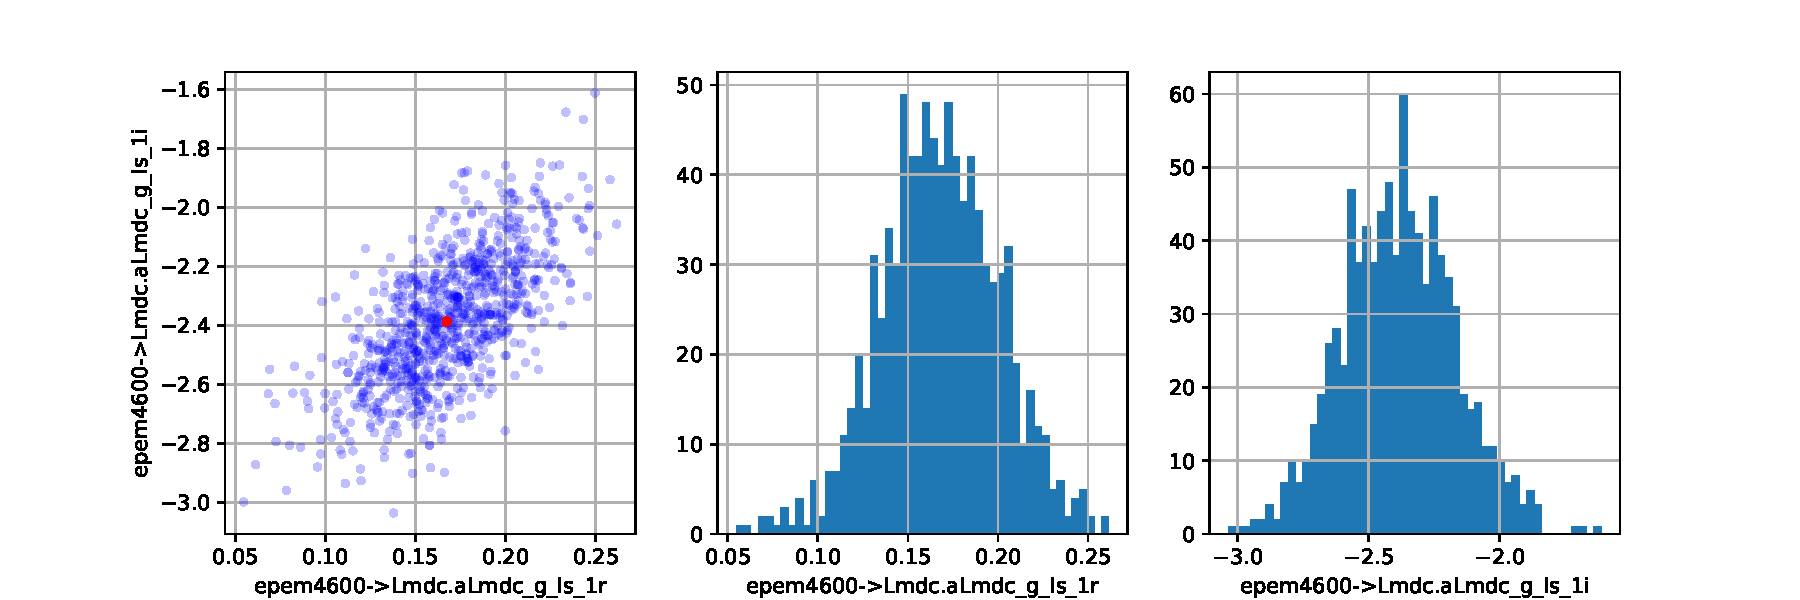
\includegraphics[width=0.90\textwidth]{figure/app_ff/sample.pdf}
    \caption{Distributions of generated two floated parameters and their correlations.}
\label{fig:gen_params} 
\end{figure}

The FFs and interference parts are calculated using Eq.~\ref{eq:ff} and Eq.~\ref{eq:ff2} for each set of generated parameters. The distributions of FFs of $\Delta(1232)^{++}$ and its interference parts with the other resonances are shown in Figure~\ref{fig:ff_delta1232} at $\sqrt{s} = 4.600\gev/c^2$. Fits are performed using a Gaussian function and fit results are listed in Table~\ref{tab:ff_delta1232}. The ratios of fit $\sigma$ values and nominal errors are found to be around 1. For the other resonances, the comparison results are the same. In conclusion, the error propagation formula, Eq.~\ref{eq:ff3}, can provide correct estimations for FF errors. 

\begin{figure}[htbp]\centering
    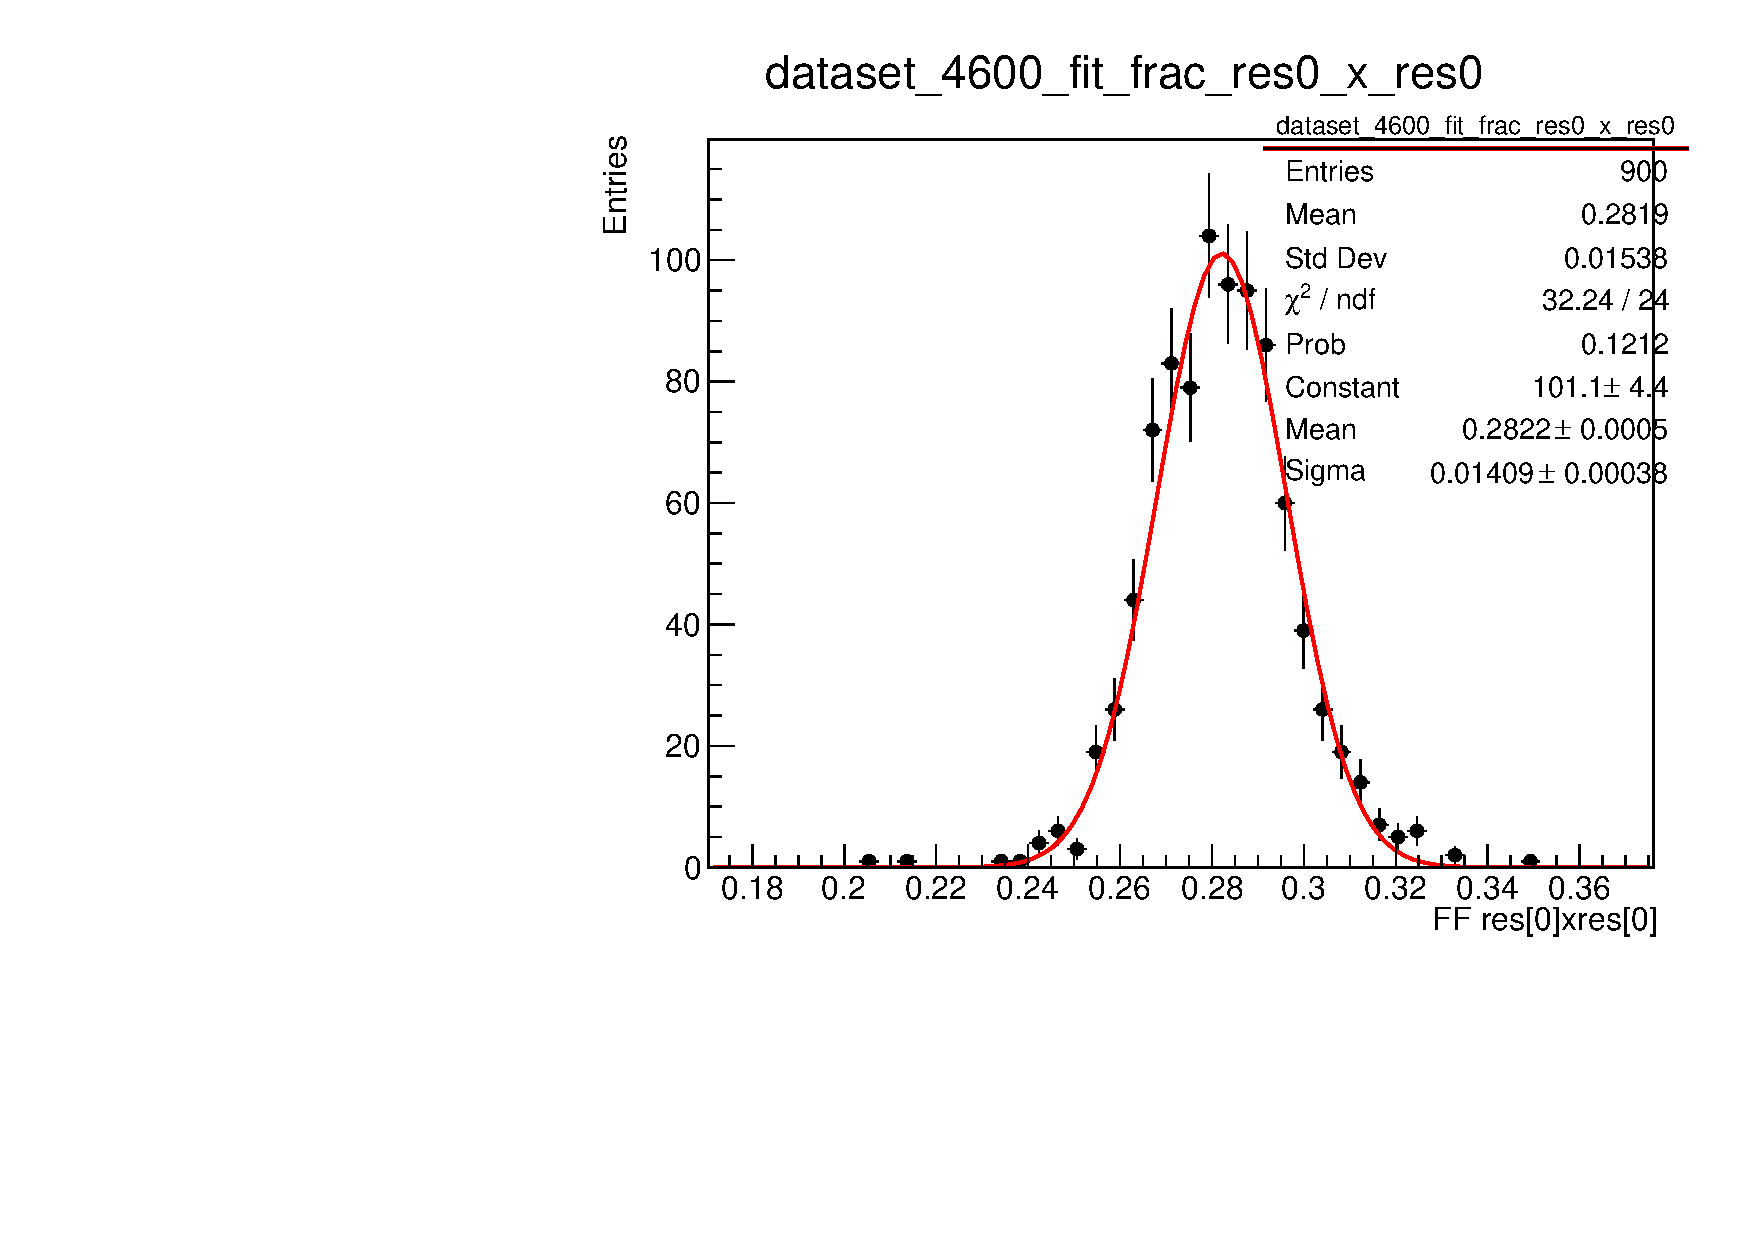
\includegraphics[width=0.24\textwidth]{figure/app_ff/dataset_4600_fit_frac_res0_x_res0.pdf}
    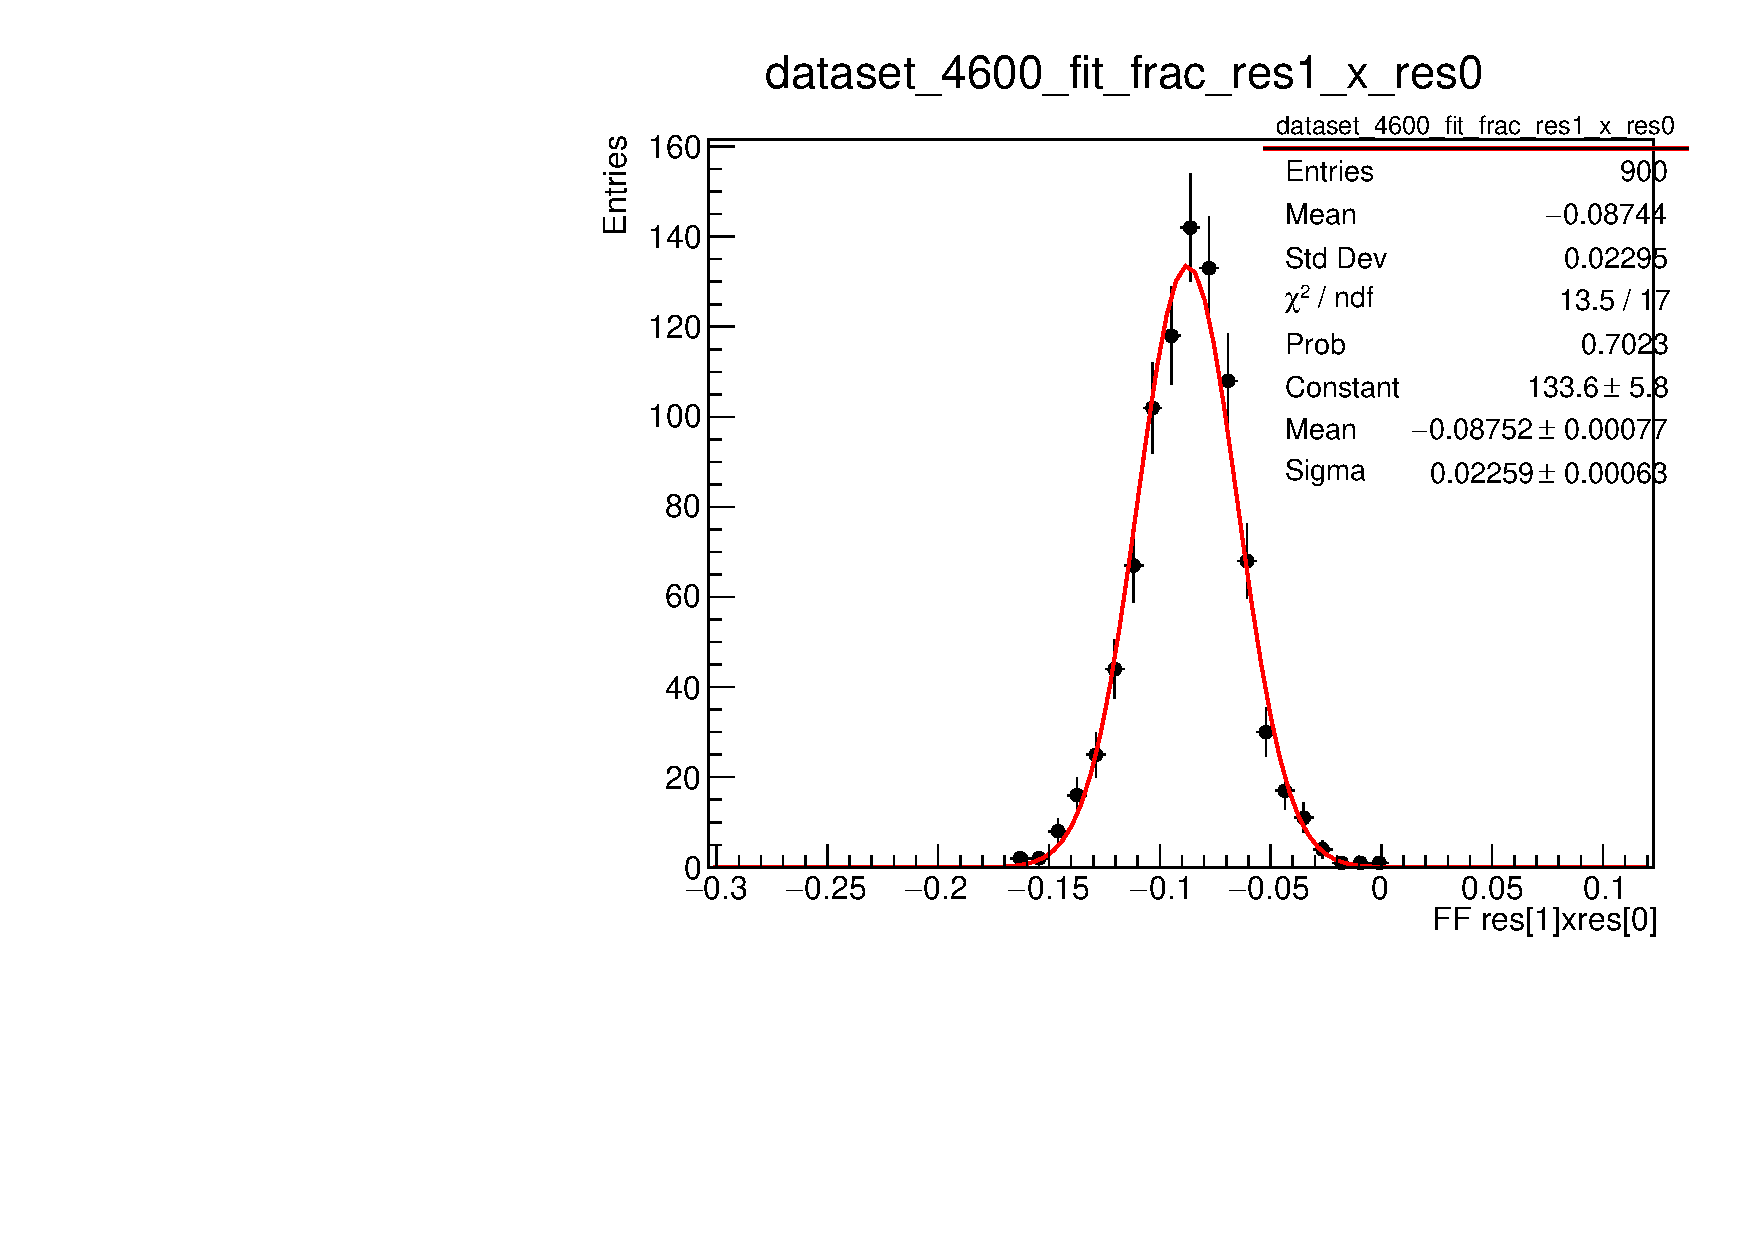
\includegraphics[width=0.24\textwidth]{figure/app_ff/dataset_4600_fit_frac_res1_x_res0.pdf}
    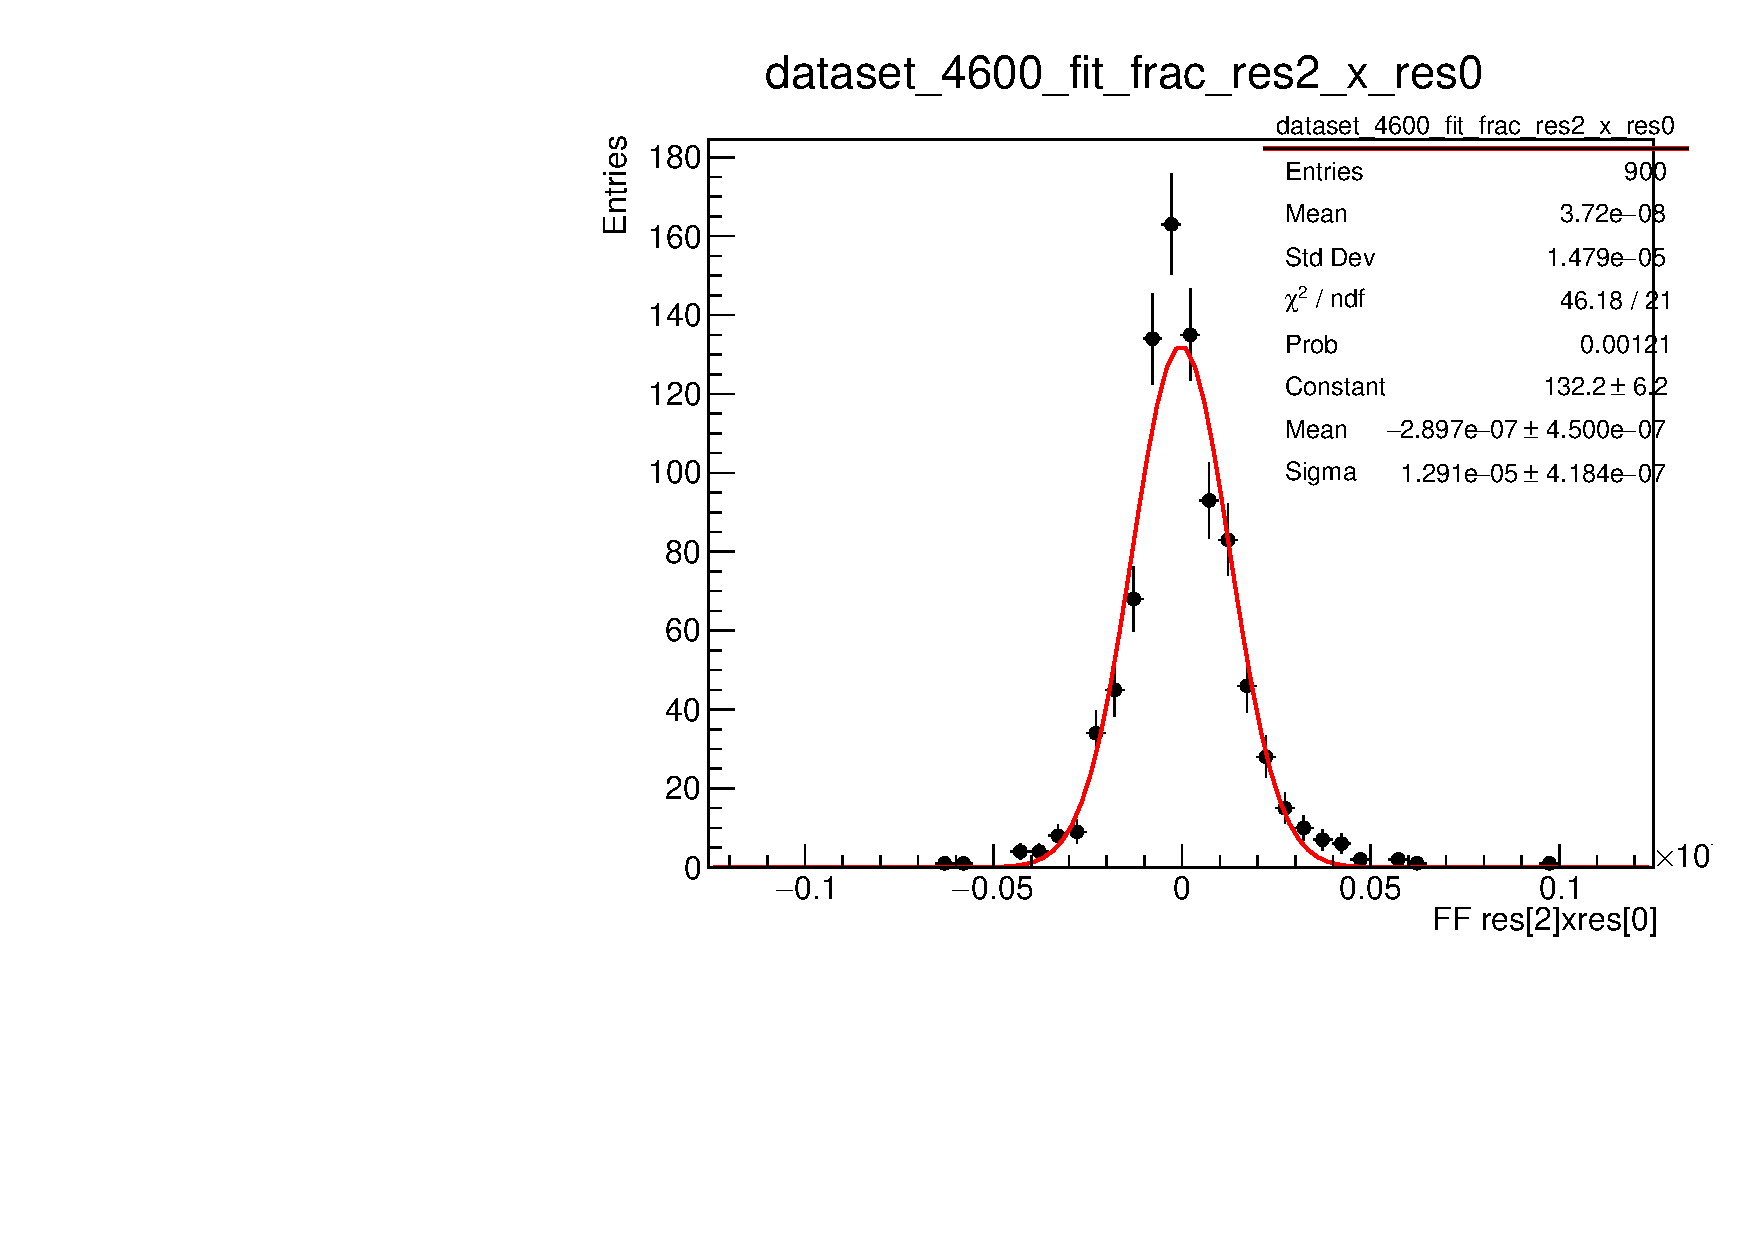
\includegraphics[width=0.24\textwidth]{figure/app_ff/dataset_4600_fit_frac_res2_x_res0.pdf}
    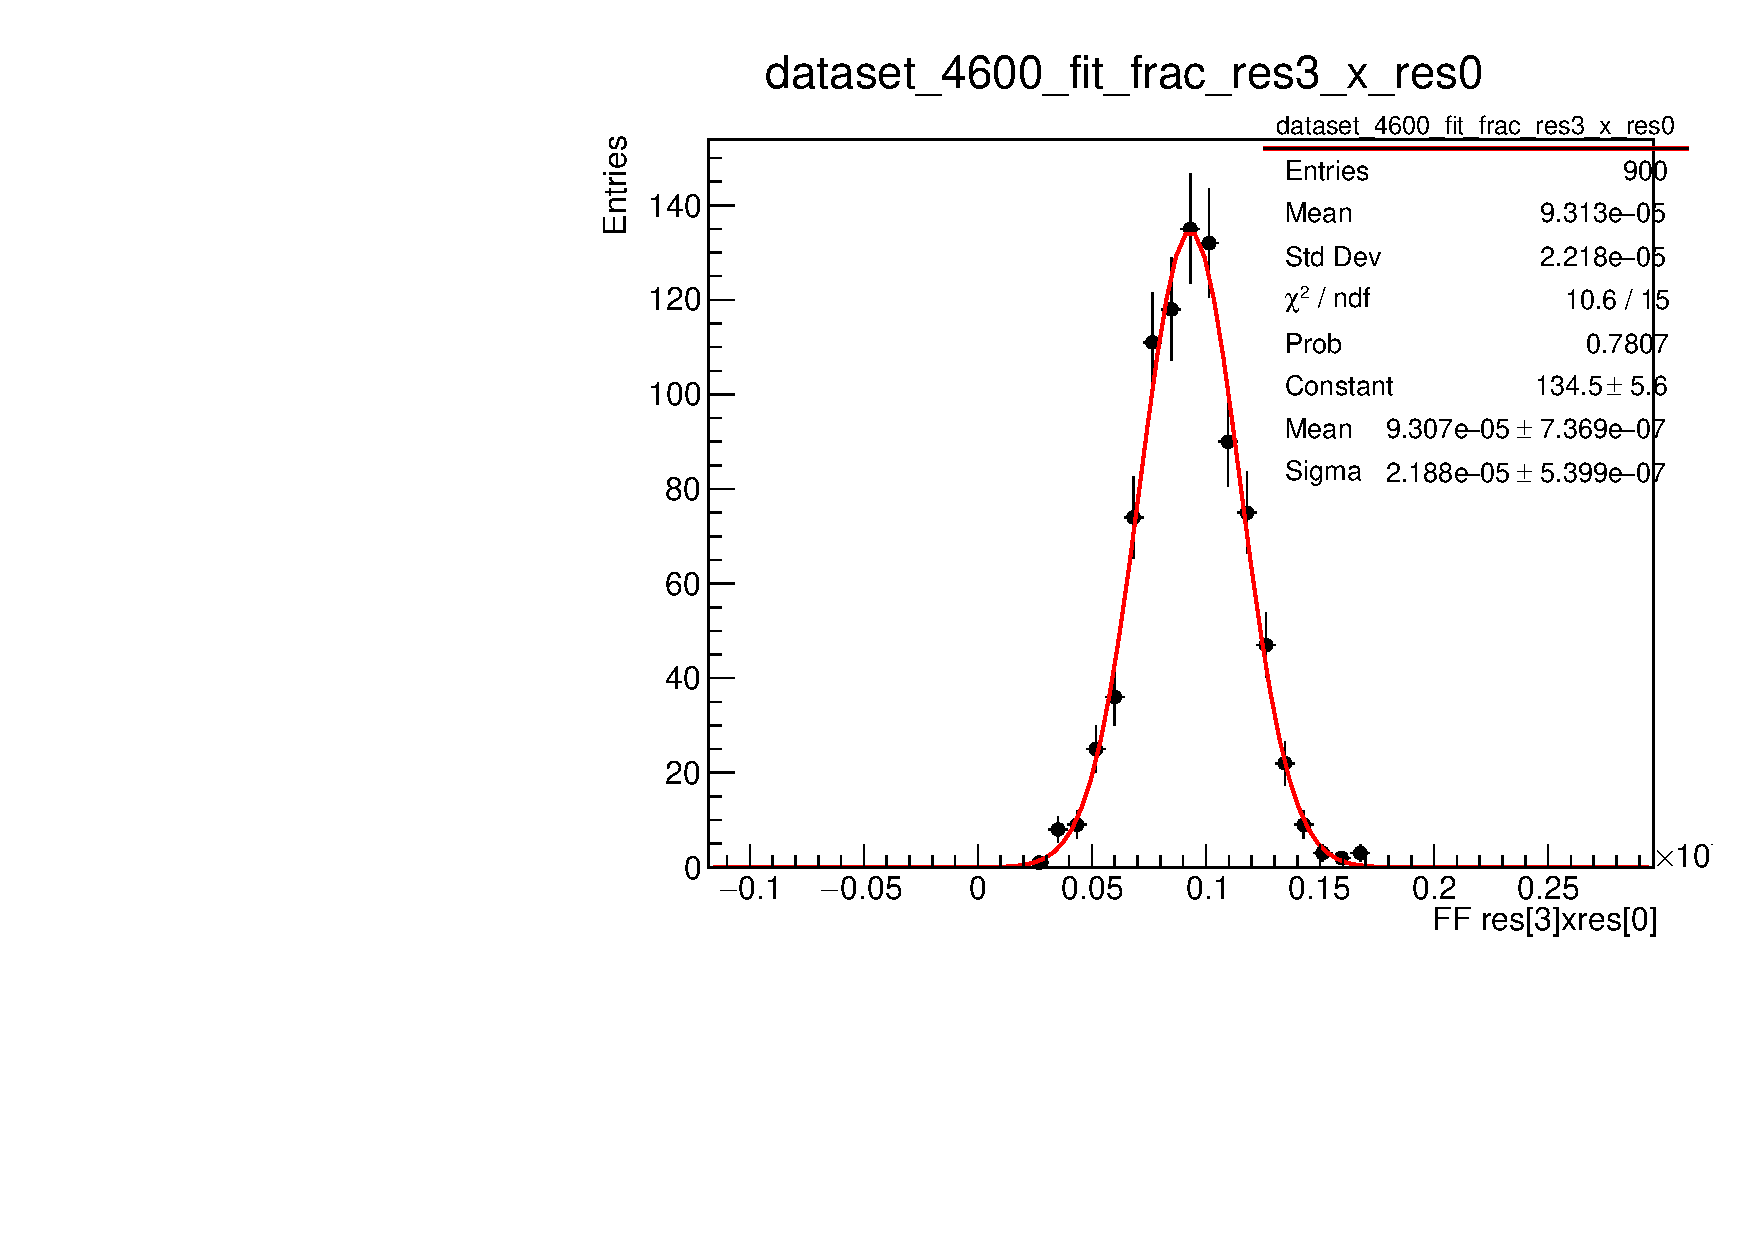
\includegraphics[width=0.24\textwidth]{figure/app_ff/dataset_4600_fit_frac_res3_x_res0.pdf}\\
    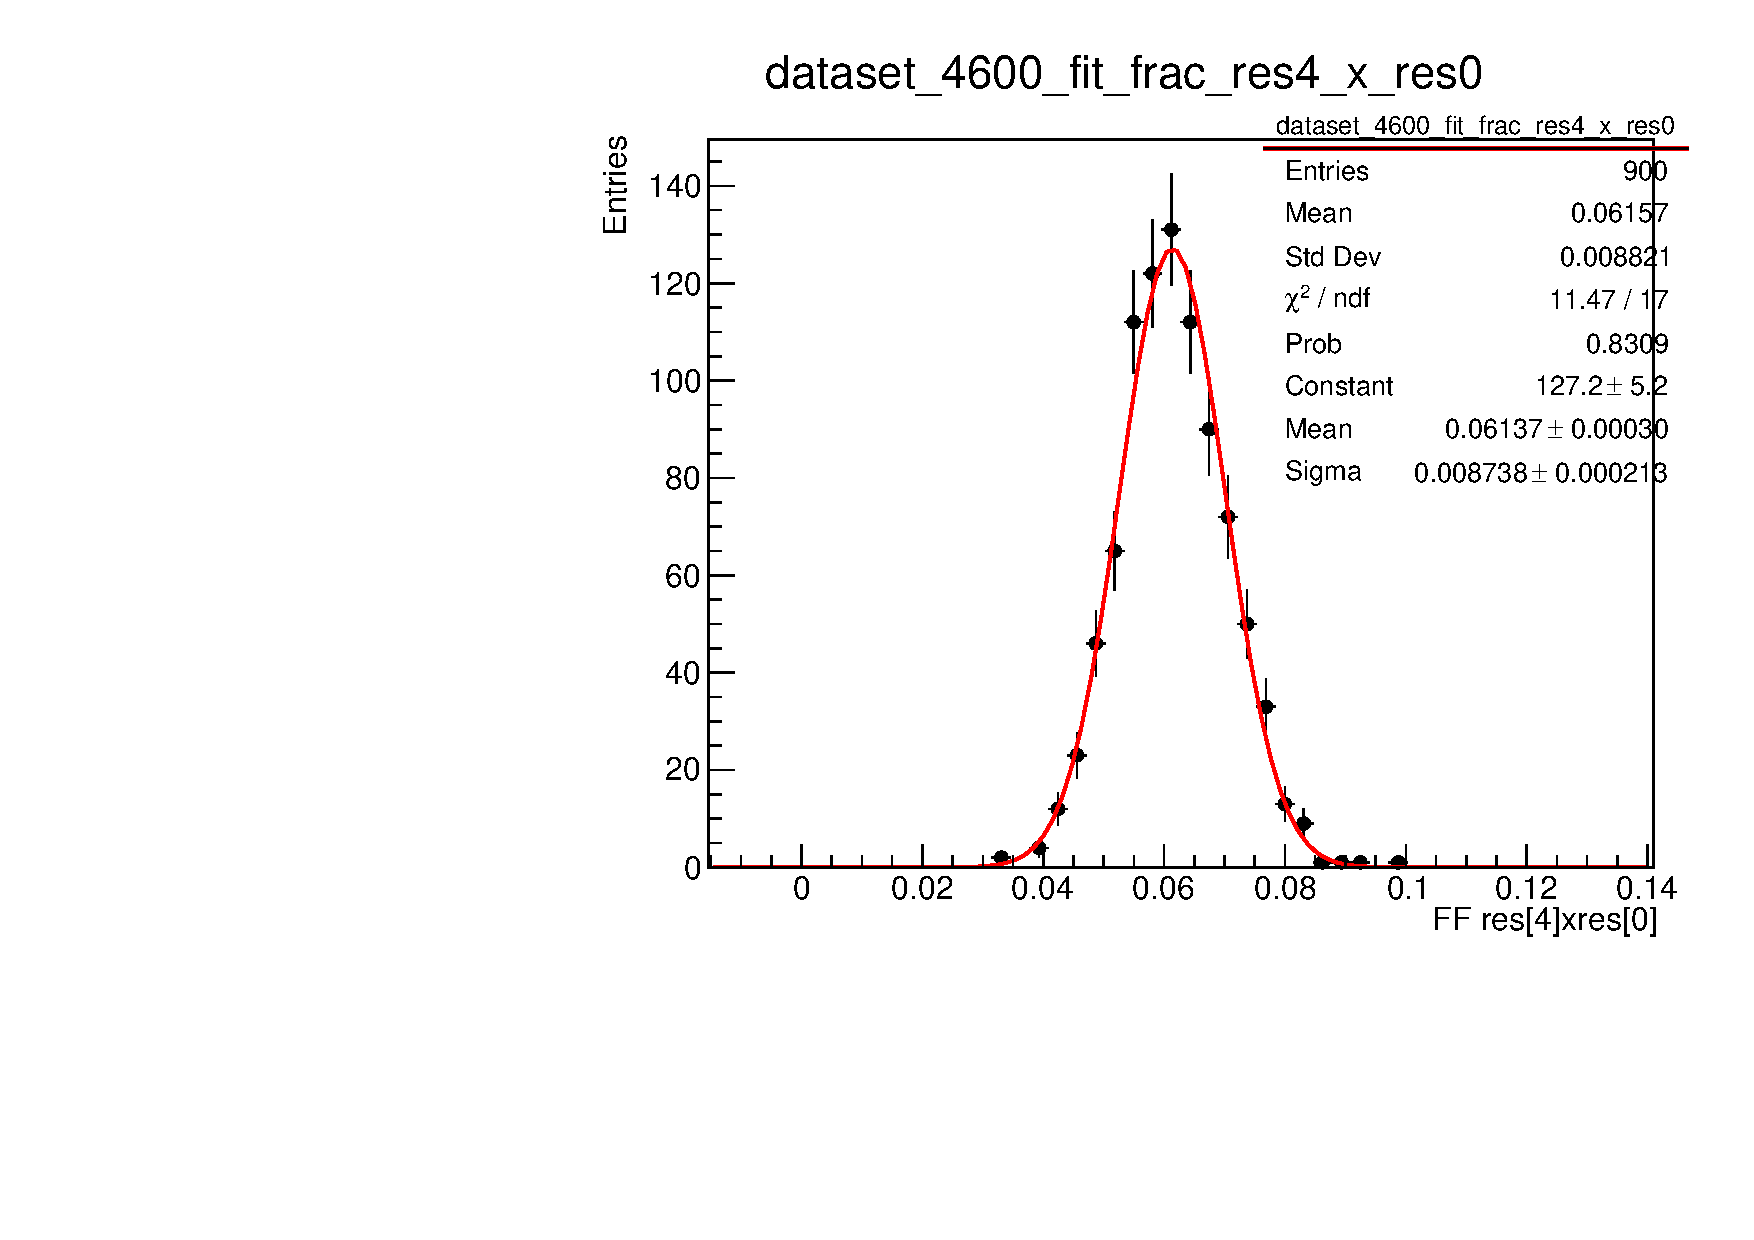
\includegraphics[width=0.24\textwidth]{figure/app_ff/dataset_4600_fit_frac_res4_x_res0.pdf}
    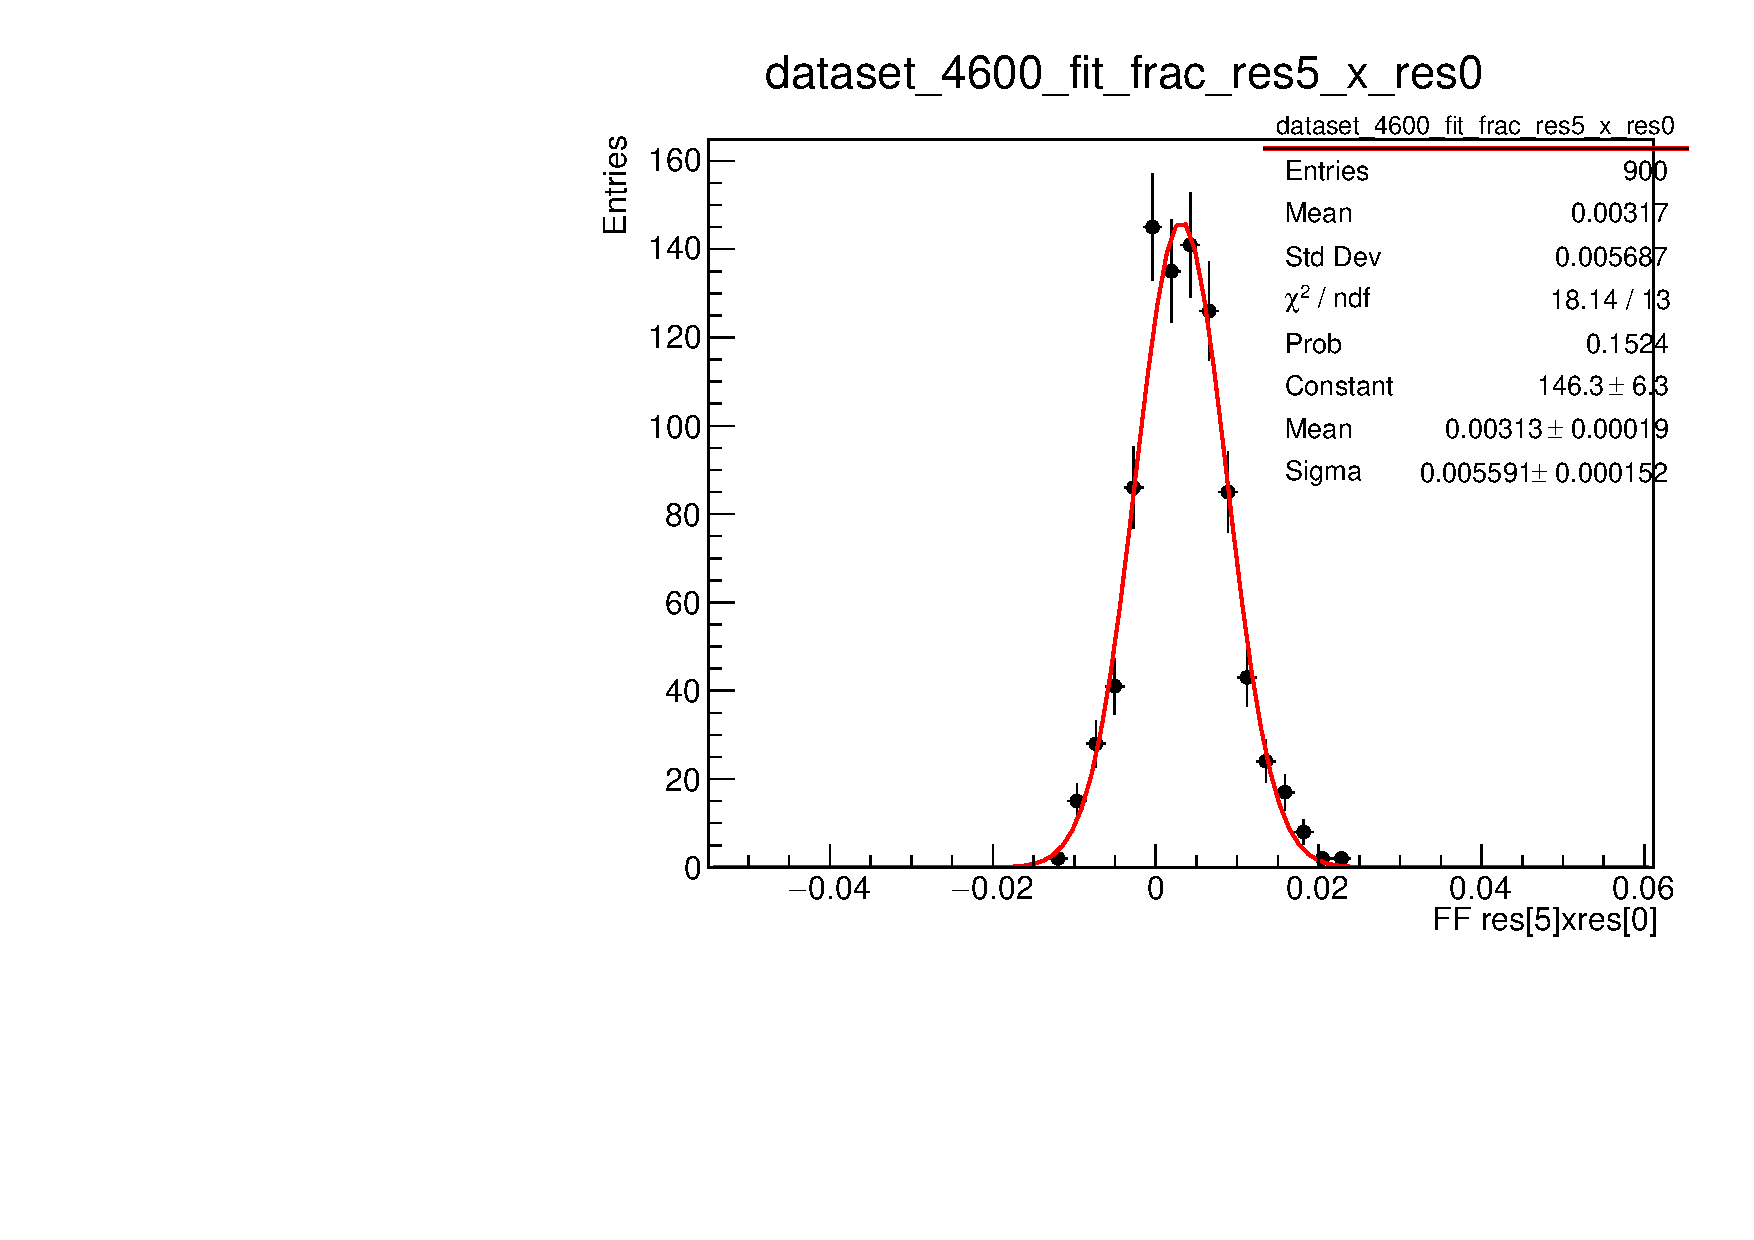
\includegraphics[width=0.24\textwidth]{figure/app_ff/dataset_4600_fit_frac_res5_x_res0.pdf}
    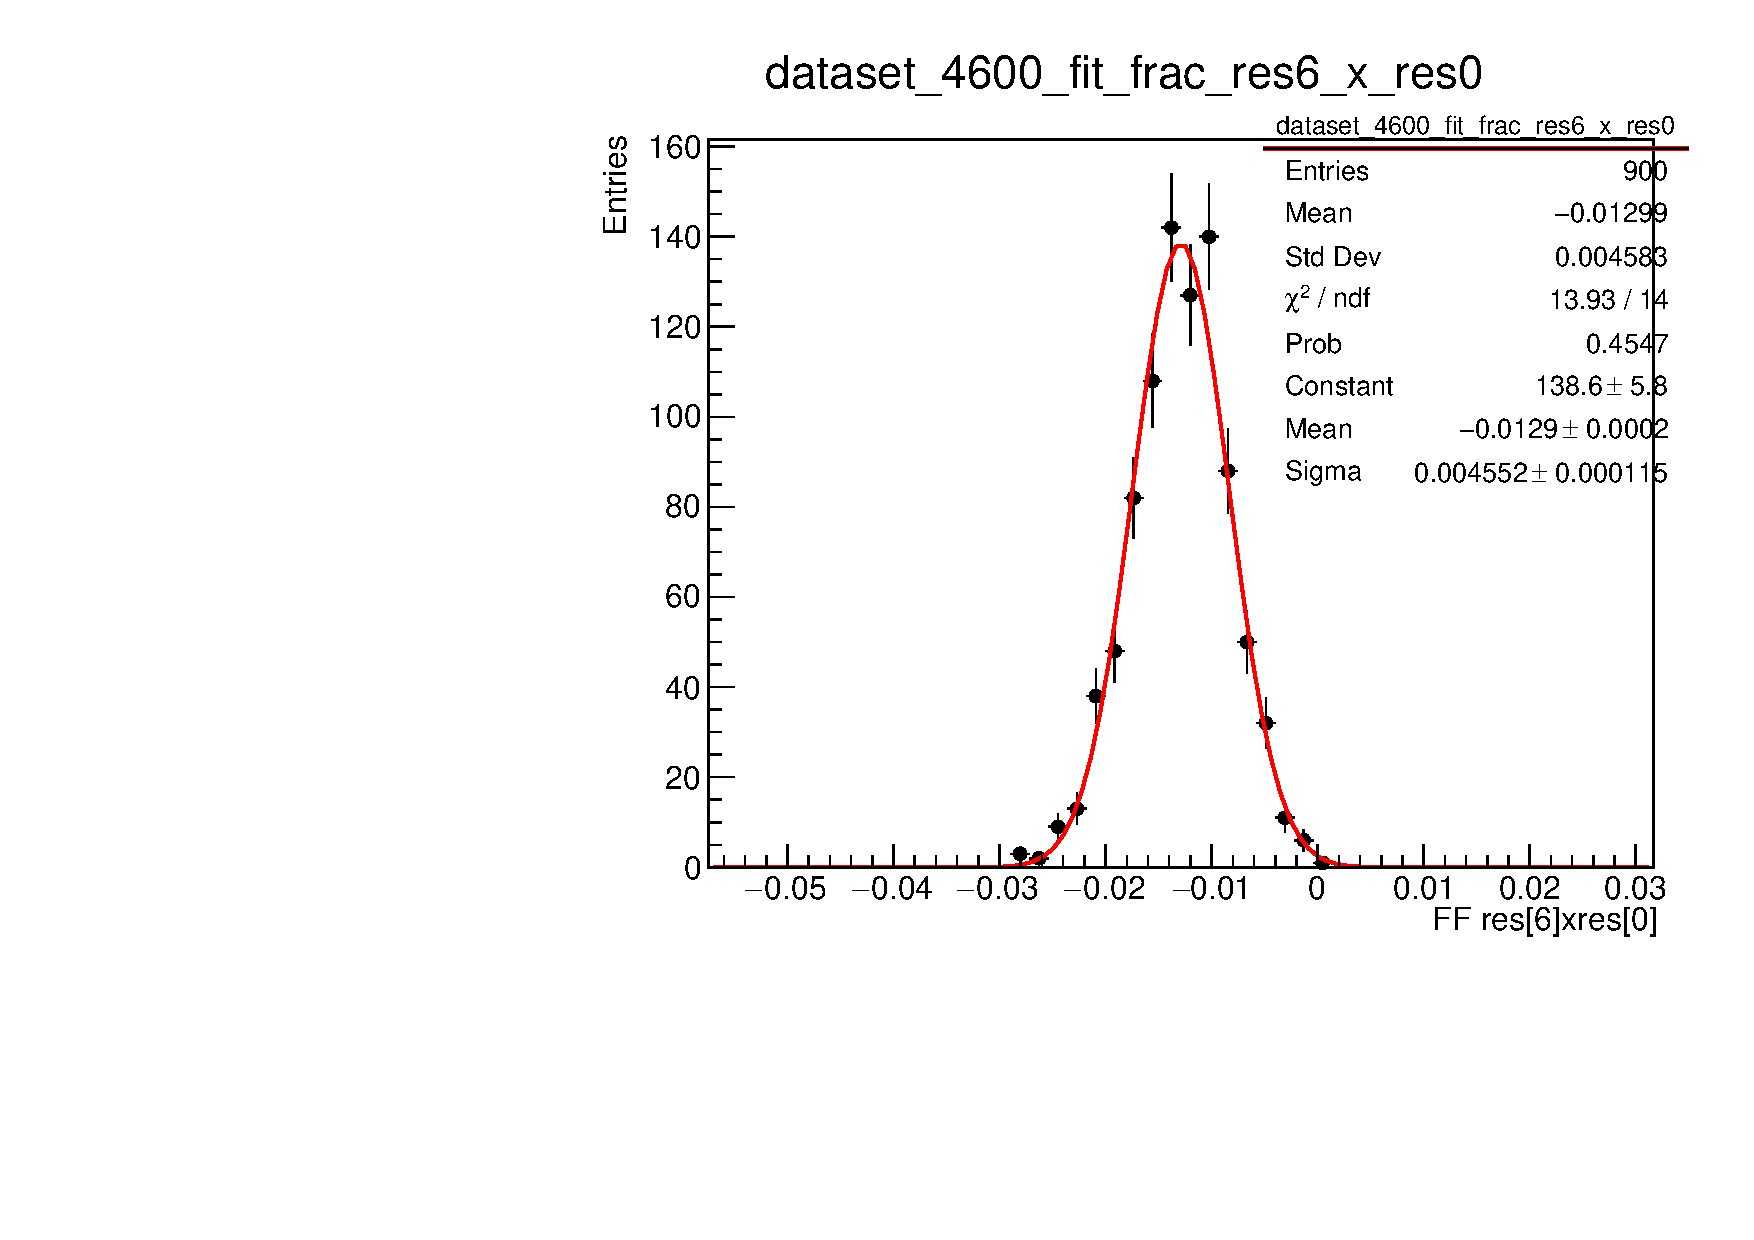
\includegraphics[width=0.24\textwidth]{figure/app_ff/dataset_4600_fit_frac_res6_x_res0.pdf}
    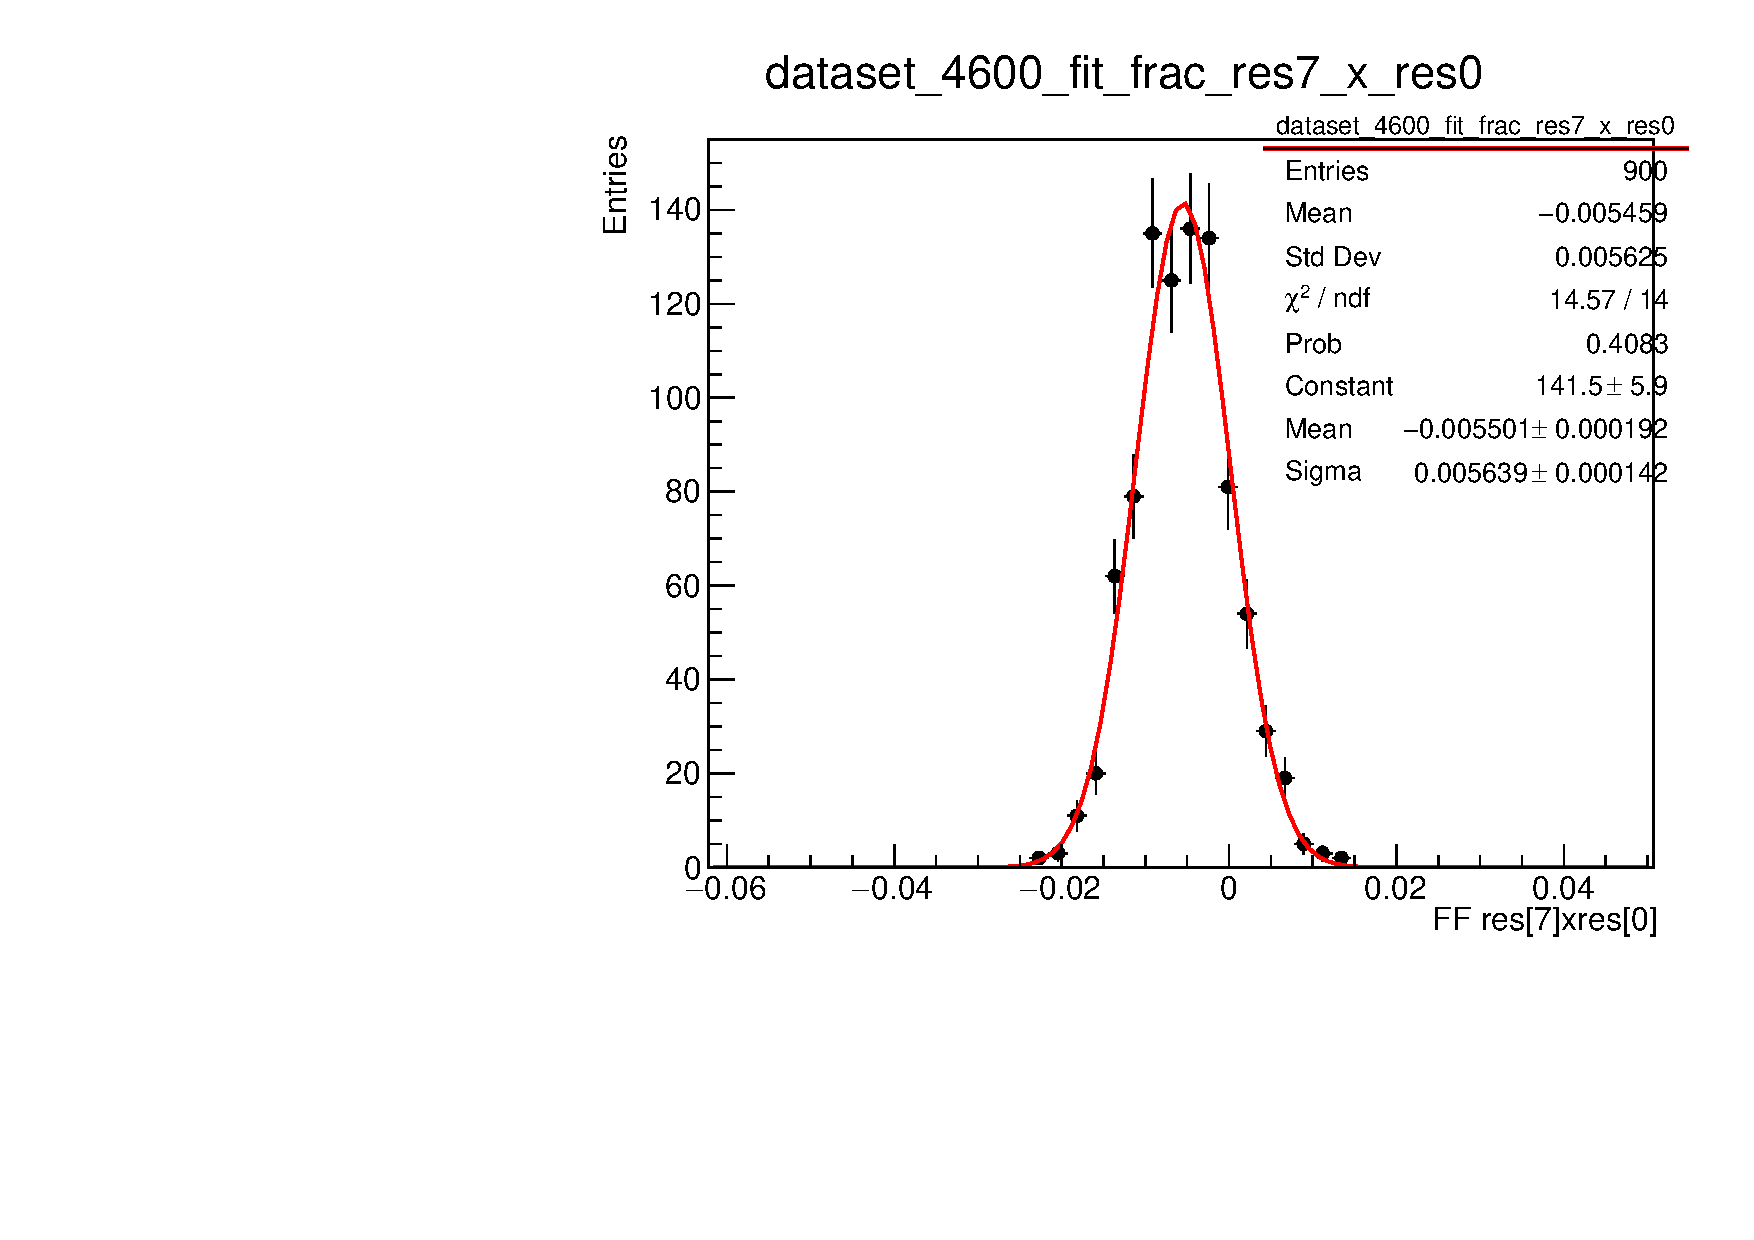
\includegraphics[width=0.24\textwidth]{figure/app_ff/dataset_4600_fit_frac_res7_x_res0.pdf} \\
    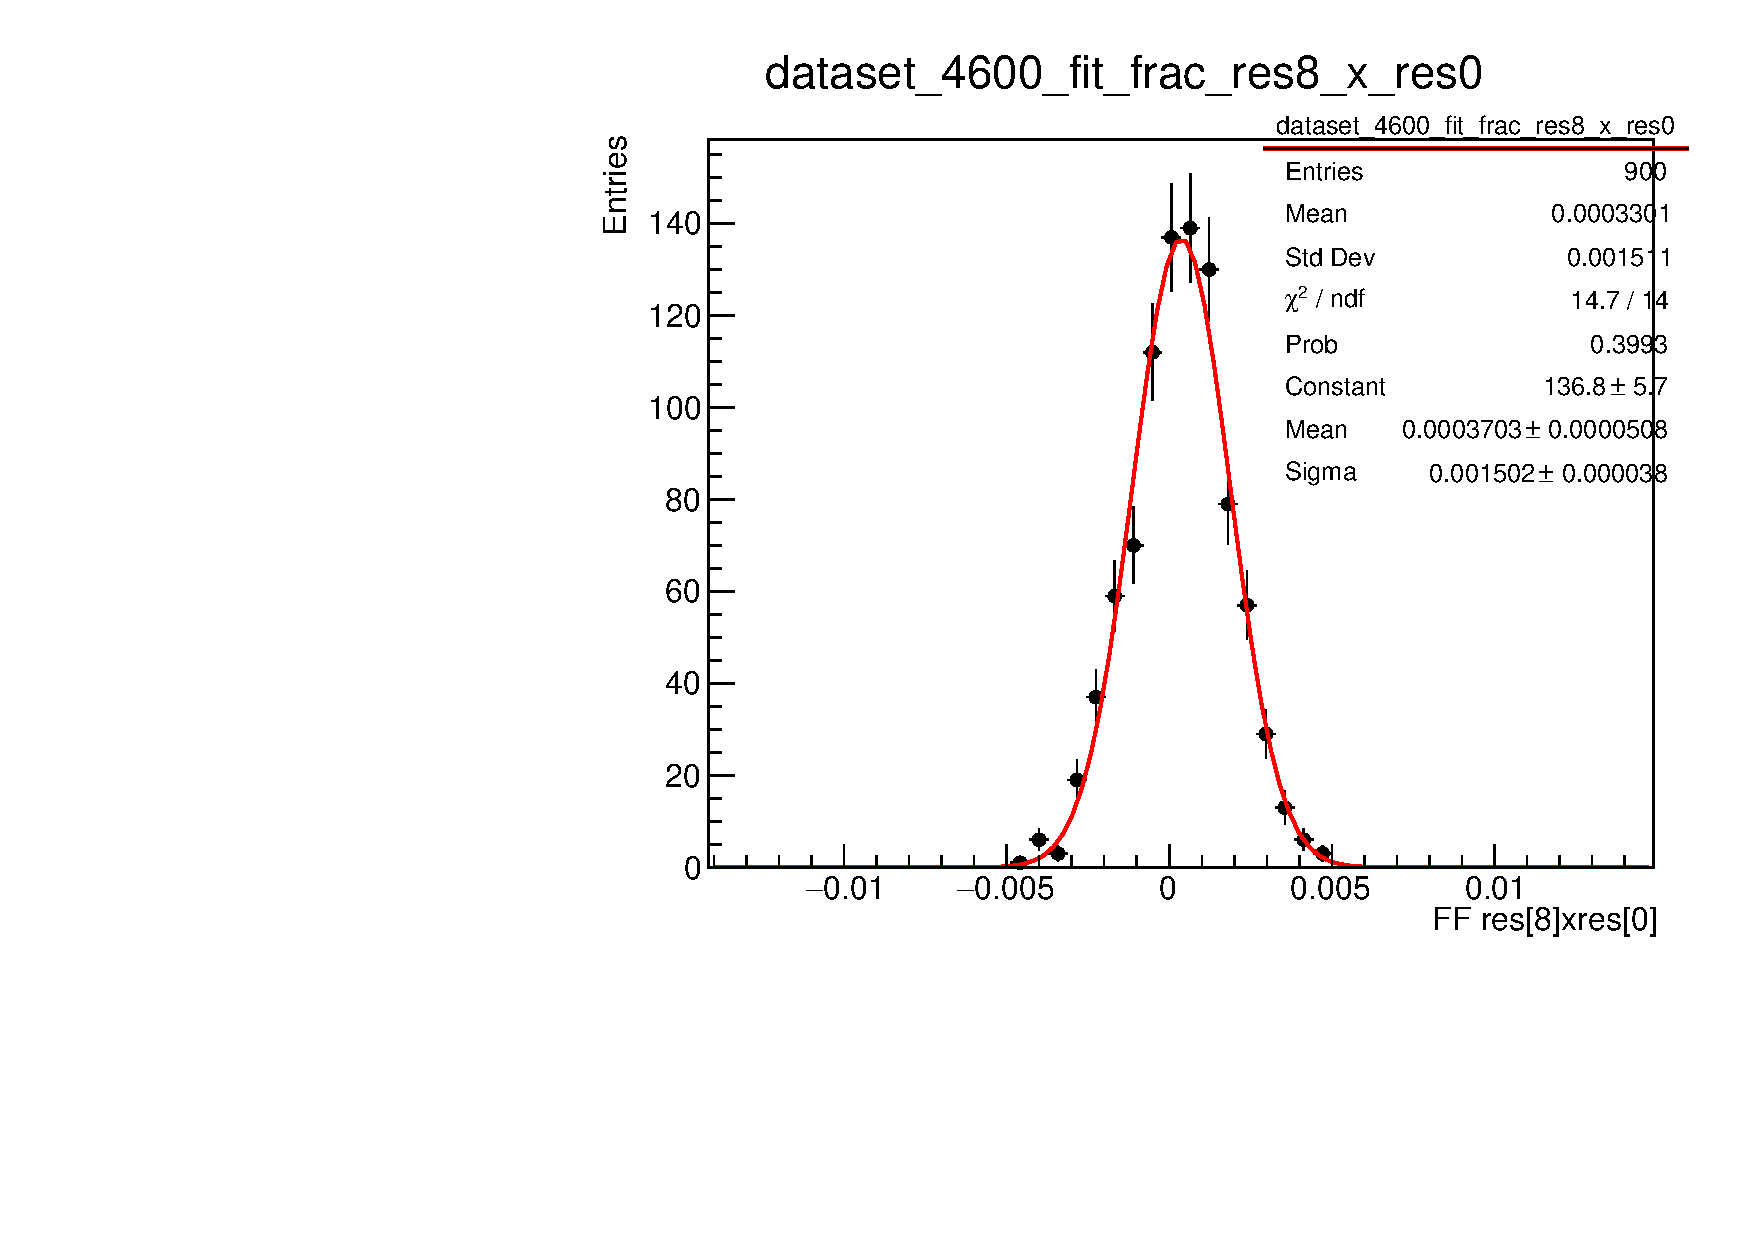
\includegraphics[width=0.24\textwidth]{figure/app_ff/dataset_4600_fit_frac_res8_x_res0.pdf}
    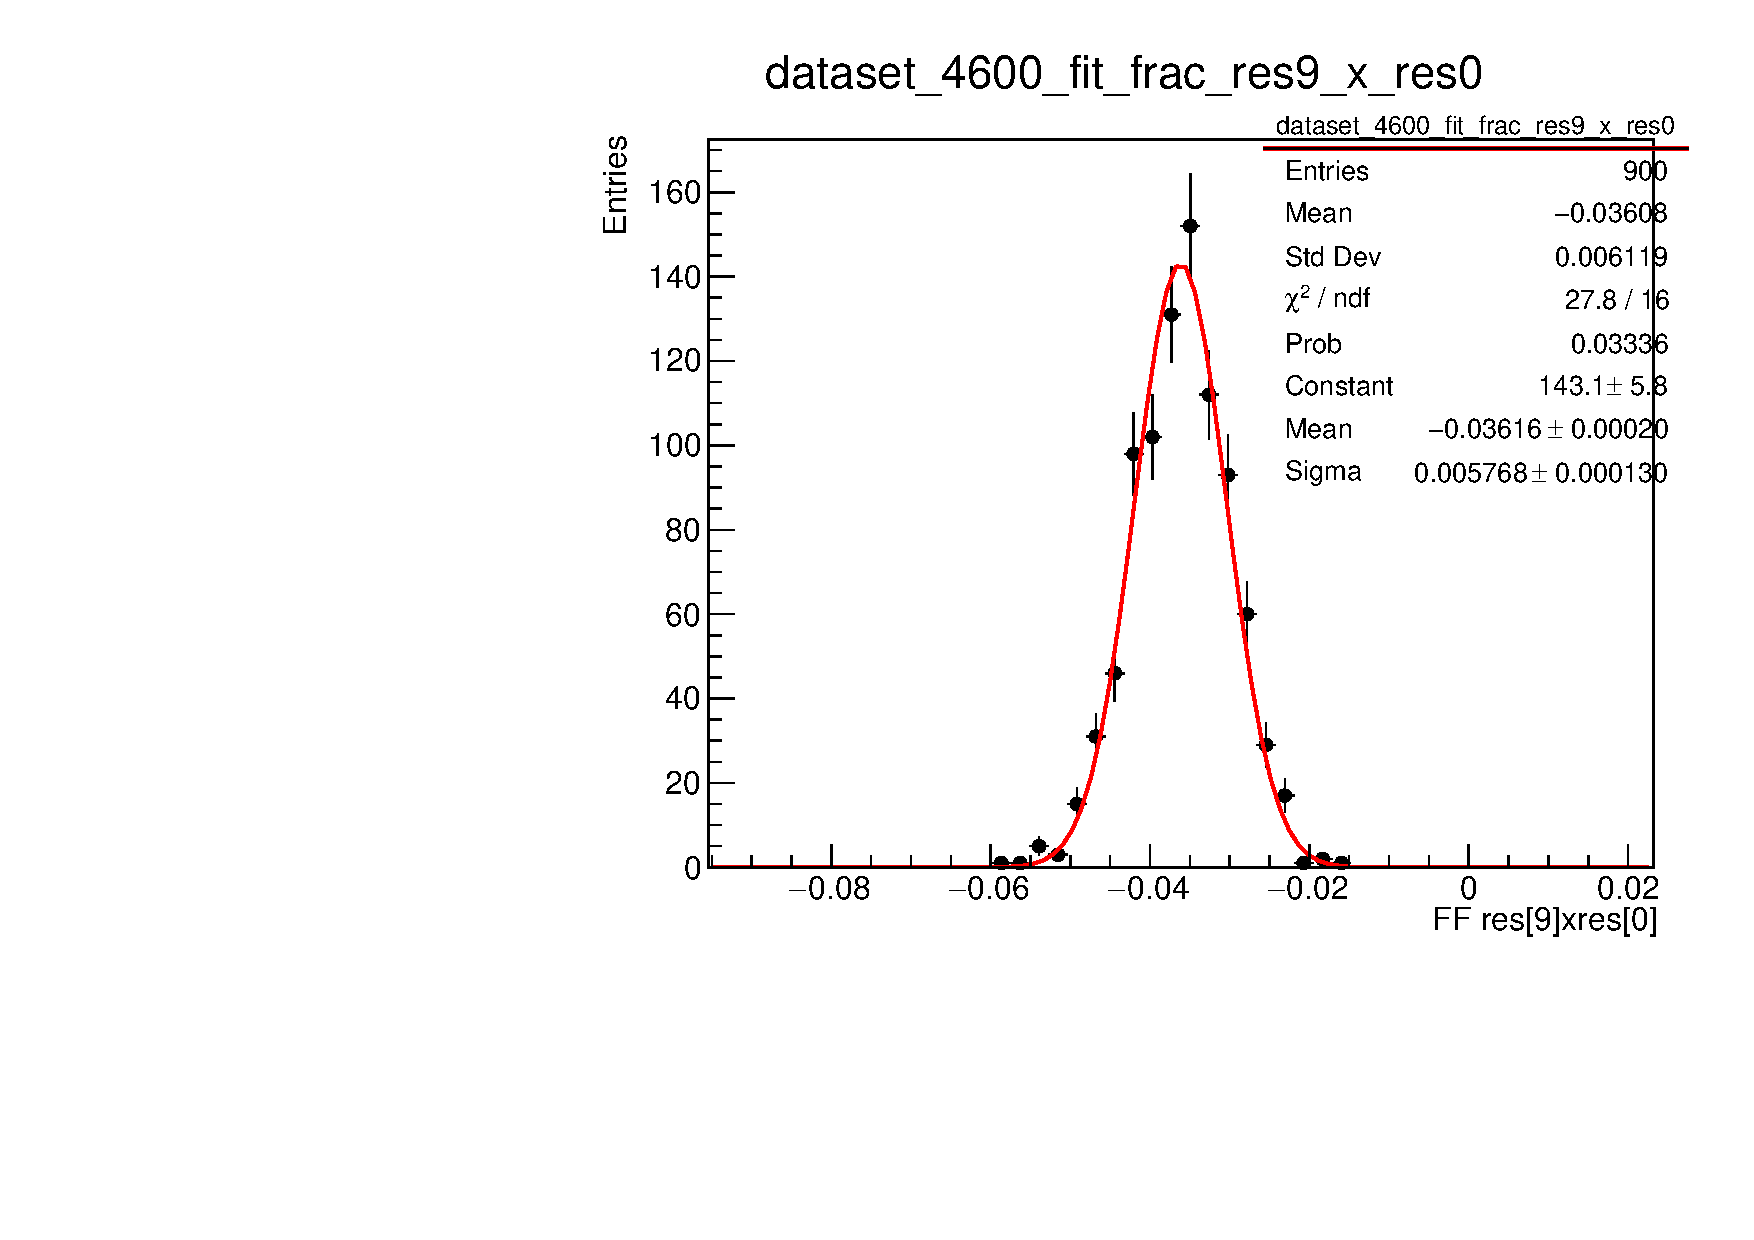
\includegraphics[width=0.24\textwidth]{figure/app_ff/dataset_4600_fit_frac_res9_x_res0.pdf}
    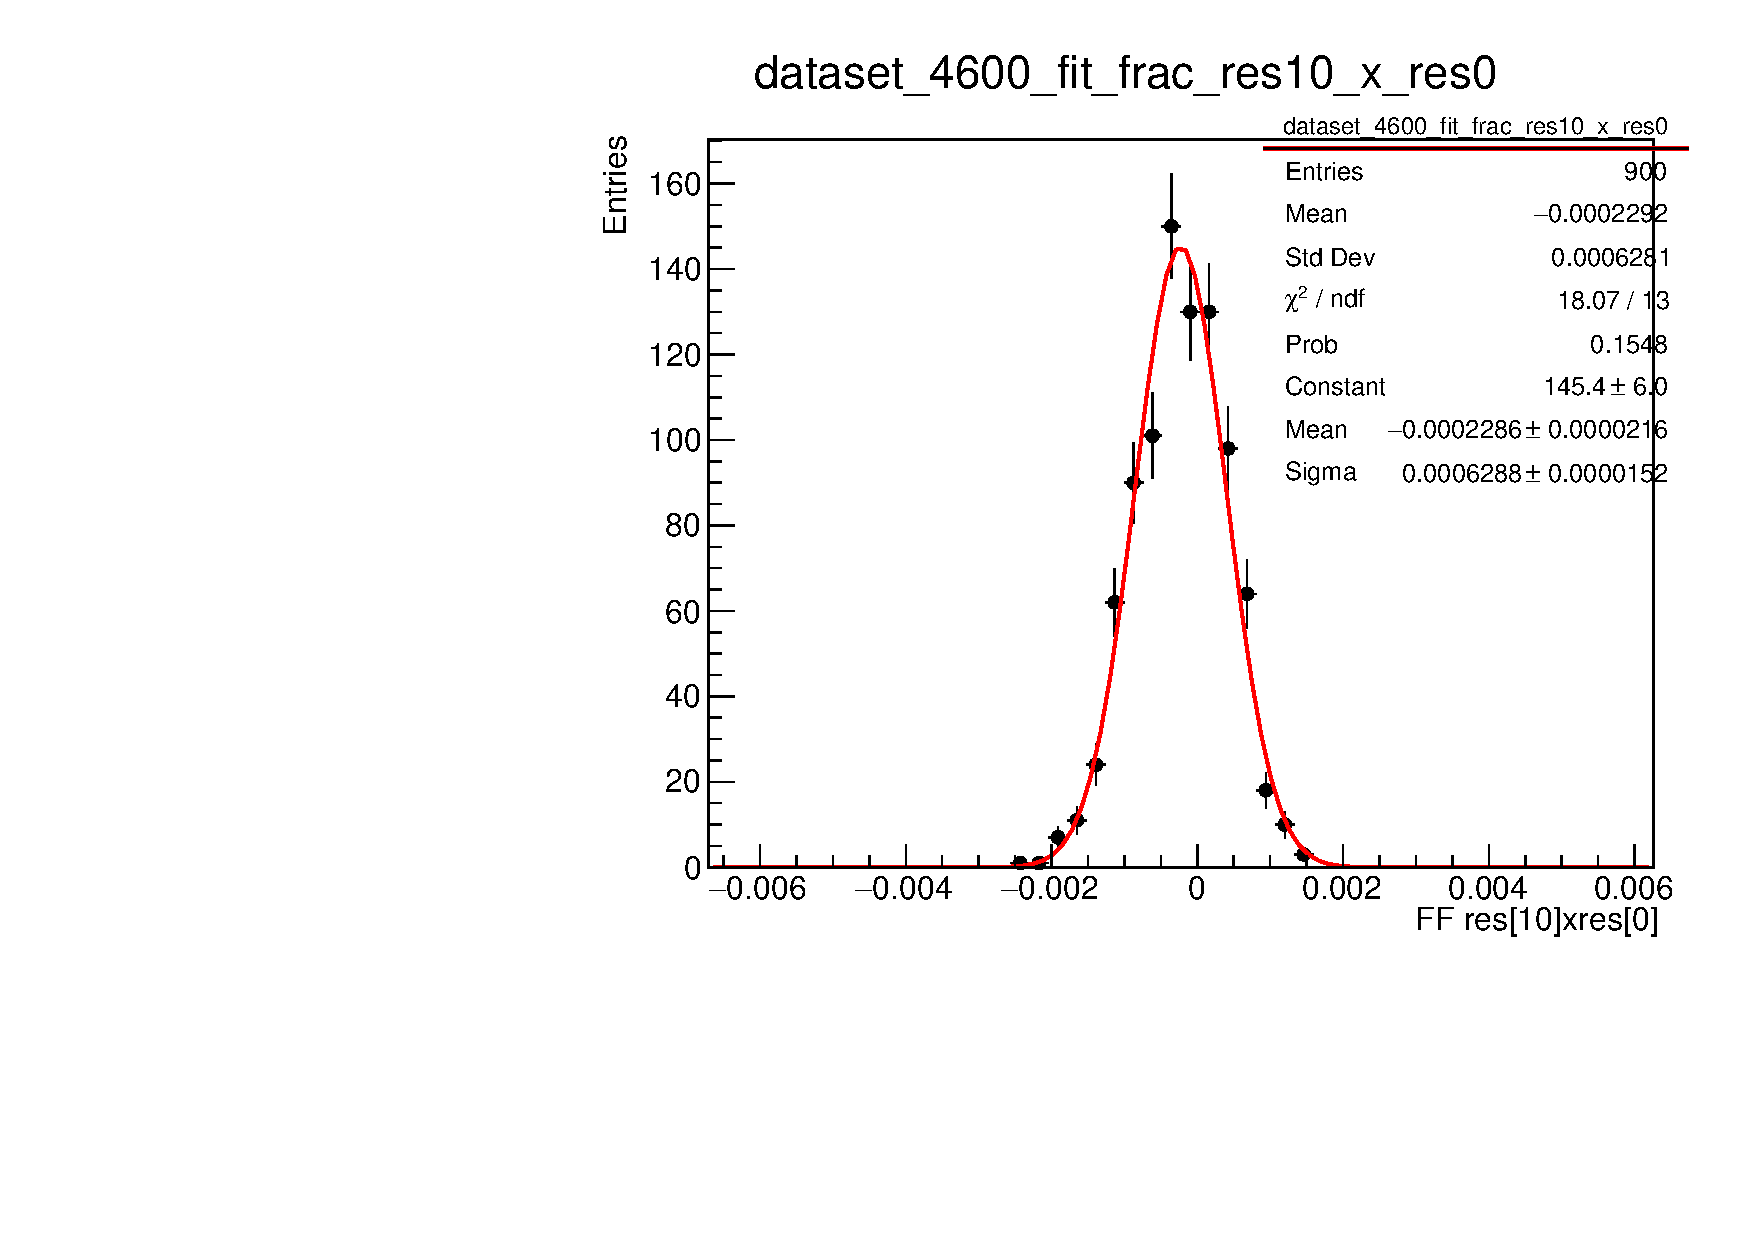
\includegraphics[width=0.24\textwidth]{figure/app_ff/dataset_4600_fit_frac_res10_x_res0.pdf}
    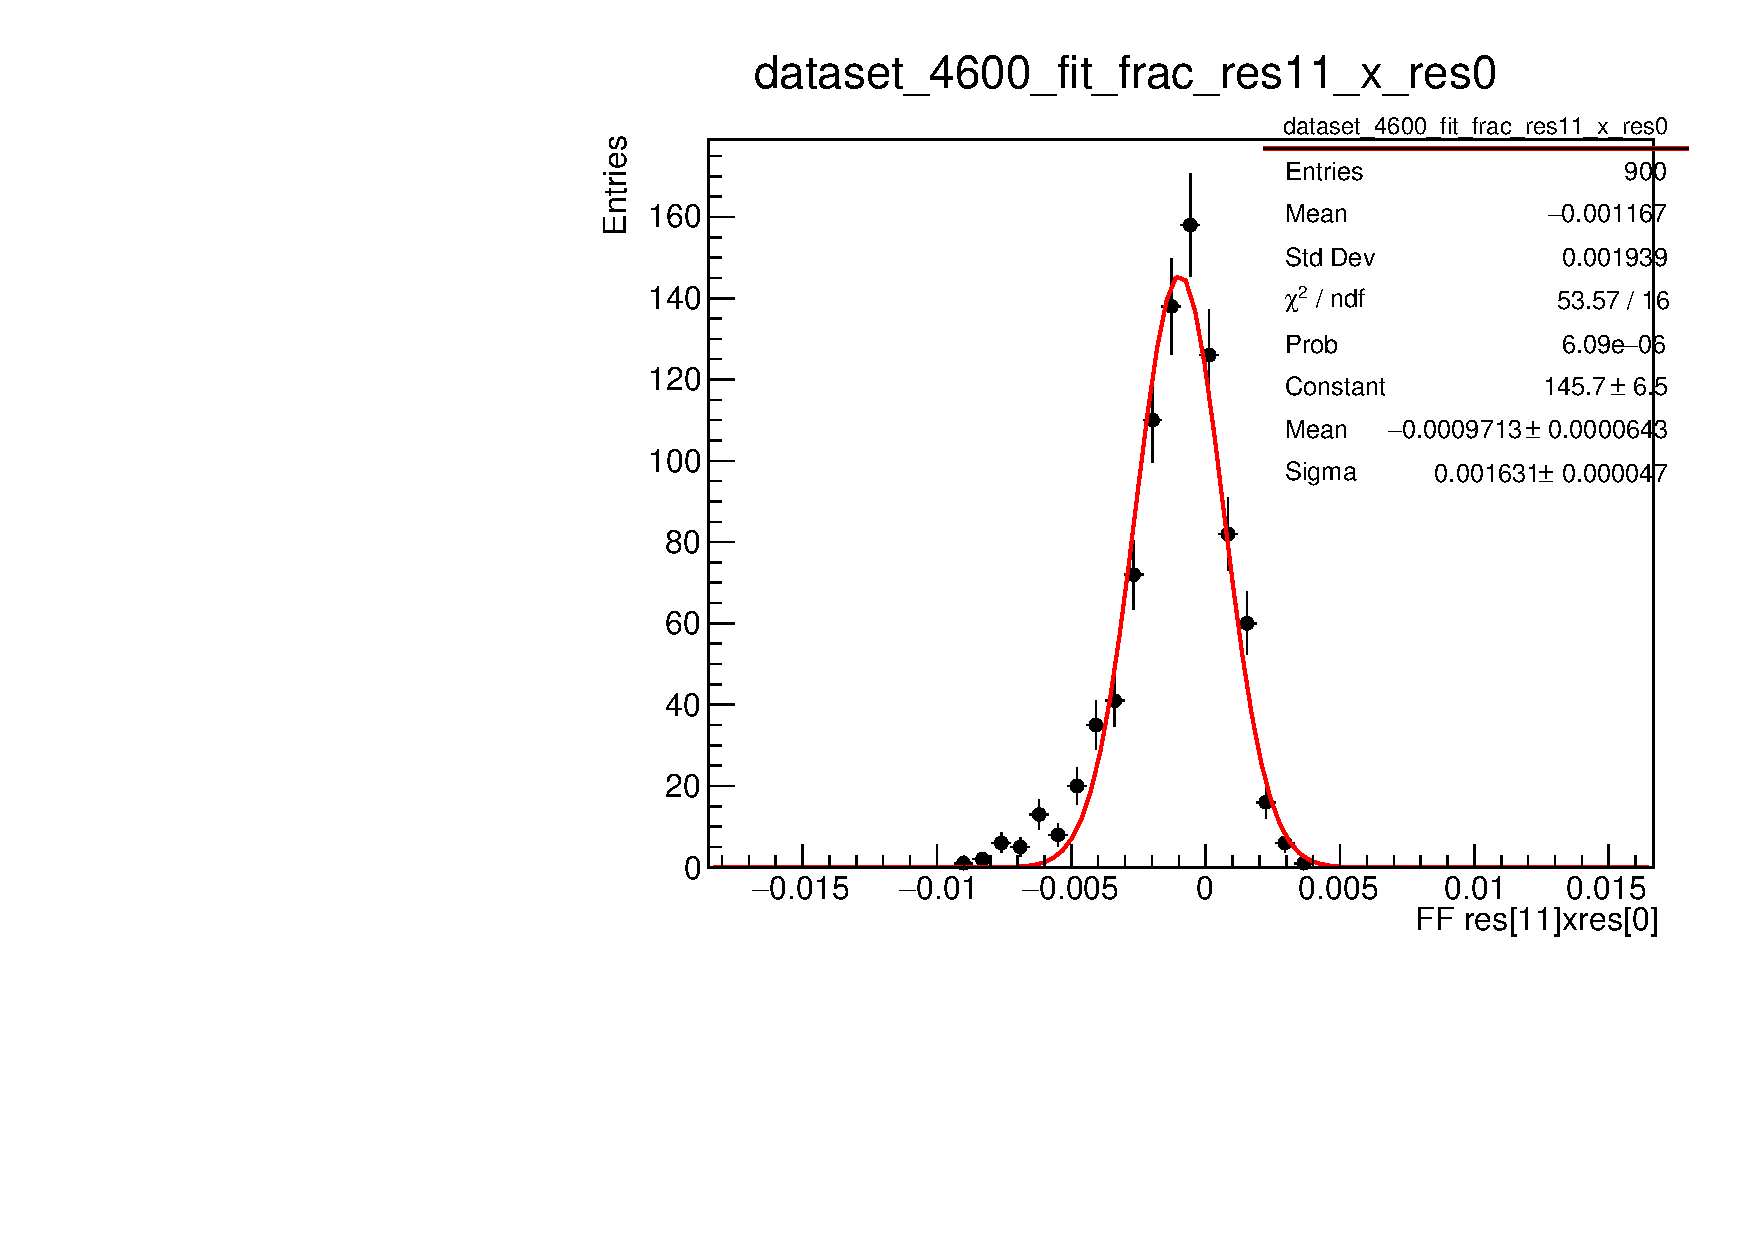
\includegraphics[width=0.24\textwidth]{figure/app_ff/dataset_4600_fit_frac_res11_x_res0.pdf} \\
    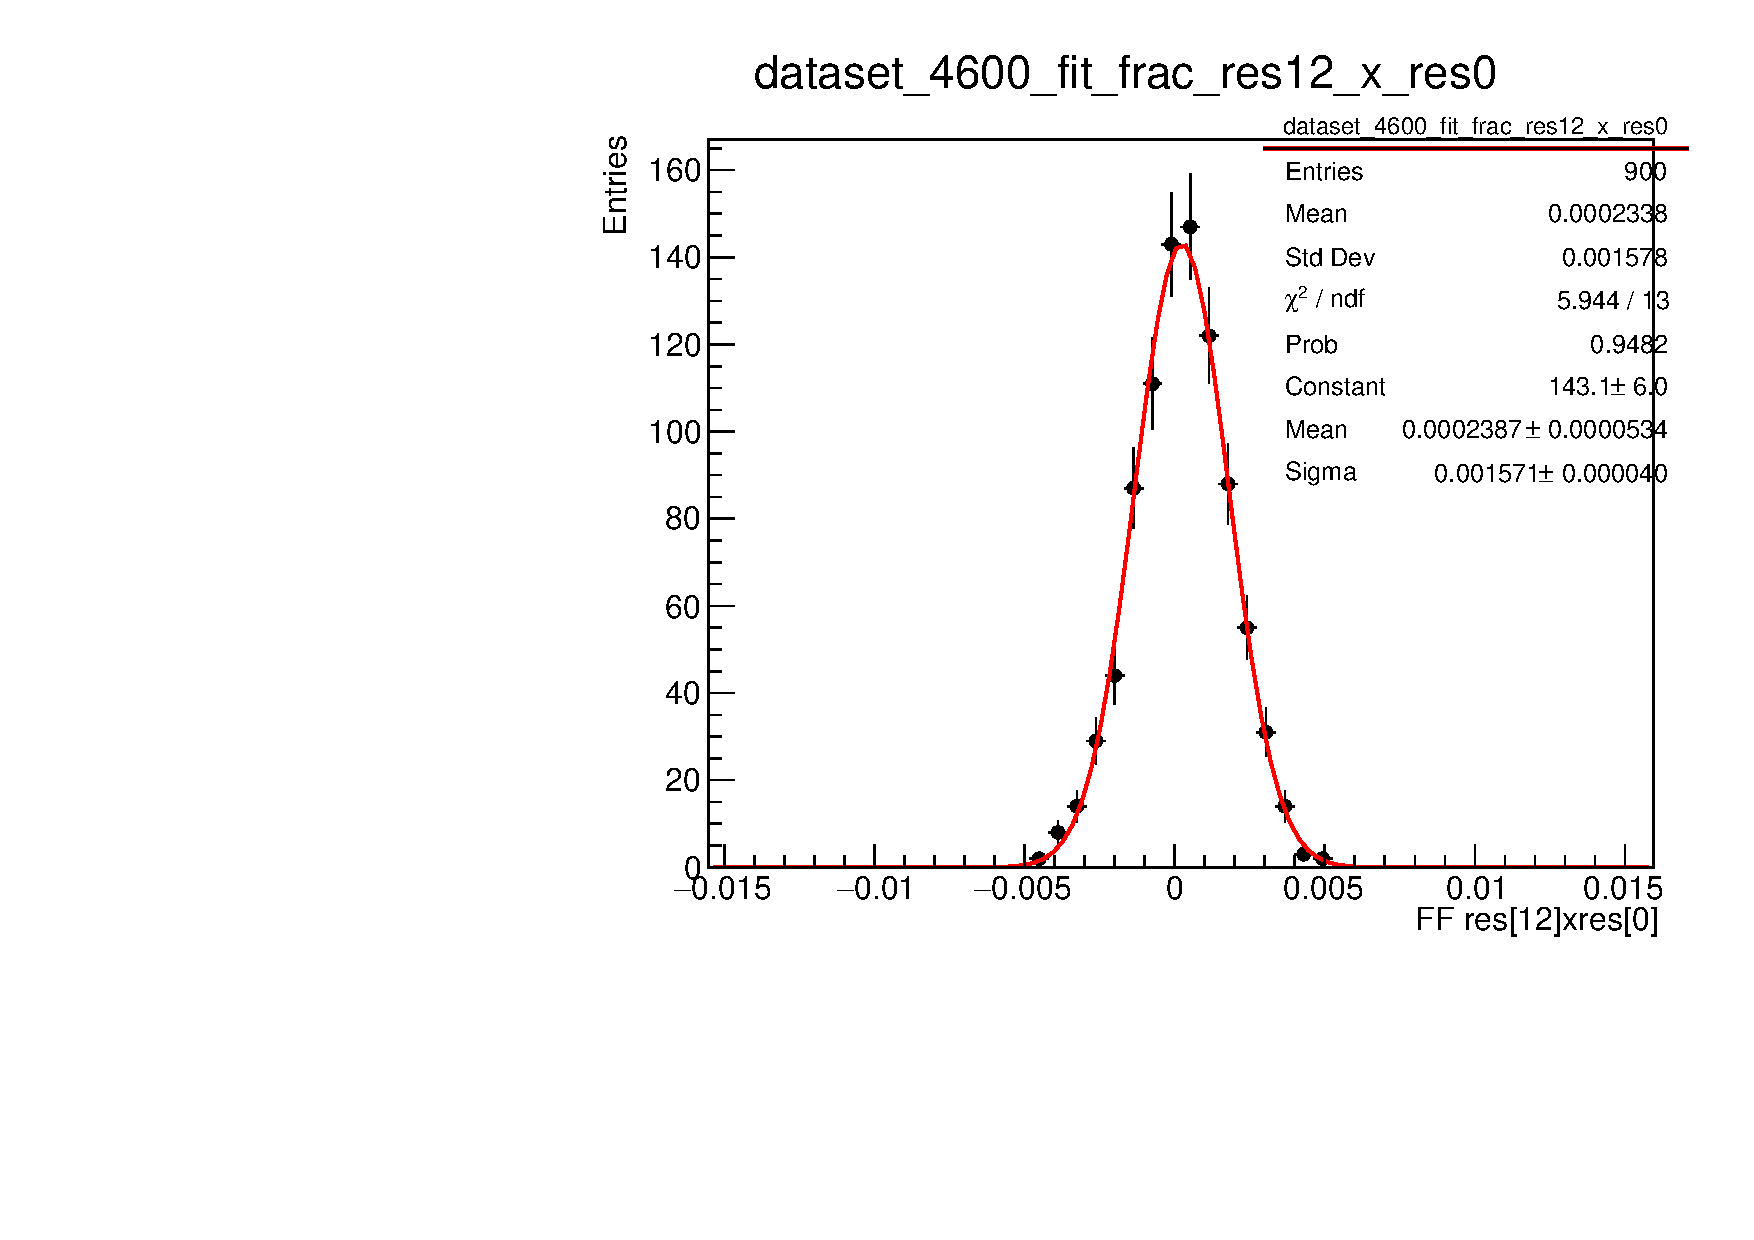
\includegraphics[width=0.24\textwidth]{figure/app_ff/dataset_4600_fit_frac_res12_x_res0.pdf}

    \caption{Distributions of FFs of $\Delta(1232)^{++}$ and its interference parts with other resonances at $\sqrt{s} = 4.600\gev/c^2$.}
\label{fig:ff_delta1232}
\end{figure}

\begin{table}[H]
    \caption{Fit results of FF distributions for $\Delta(1232)^{++}$ and comparison with nominal results.}
    \label{tab:ff_delta1232}
    \resizebox{\textwidth}{!}{
        \begin{tabular}{ccccc}
            \hline\hline
            Resonance & Nominal FF (\%) & Fit $\mu$ (\%) & Fit $\sigma$ (\%) &  Fit $\sigma$/nominal error \\\hline
            $\Delta(1232)^{++}$ & 27.3234$\pm$1.0280 & 28.2163$\pm$0.0494 & 1.4089$\pm$0.0381 & 1.371\\
            $\Delta(1600)^{++} \times \Delta(1232)^{++}$ & -9.0492$\pm$2.1321 & -8.7518$\pm$0.0772 & 2.2585$\pm$0.0626 & 1.059\\
            $\Delta(1600)^{++} \times \Delta(1232)^{++}$ & -0.0000$\pm$0.0013 & -0.0000$\pm$0.0000 & 0.0013$\pm$0.0000 & 1.031\\
            $\Delta(1700)^{++} \times \Delta(1232)^{++}$ & 0.0089$\pm$0.0021 & 0.0093$\pm$0.0001 & 0.0022$\pm$0.0001 & 1.056\\
            $\overline{K}_{0}^{*}(1430) \times \Delta(1232)^{++}$ & 6.2770$\pm$0.7818 & 6.1367$\pm$0.0296 & 0.8738$\pm$0.0213 & 1.118\\
            $\overline{K}_{0}^{*}(700) \times \Delta(1232)^{++}$ & 0.3083$\pm$0.5800 & 0.3130$\pm$0.0192 & 0.5591$\pm$0.0152 & 0.964\\
            $\overline{K^{*}}(892) \times \Delta(1232)^{++}$ & -1.2900$\pm$0.4456 & -1.2903$\pm$0.0156 & 0.4552$\pm$0.0115 & 1.022\\
            $\Lambda(1405) \times \Delta(1232)^{++}$ & -0.5757$\pm$0.5645 & -0.5501$\pm$0.0192 & 0.5639$\pm$0.0142 & 0.999\\
            $\Lambda(1520) \times \Delta(1232)^{++}$ & 0.0356$\pm$0.1452 & 0.0370$\pm$0.0051 & 0.1502$\pm$0.0038 & 1.034\\
            $\Lambda(1600) \times \Delta(1232)^{++}$ & -3.6131$\pm$0.5930 & -3.6160$\pm$0.0202 & 0.5768$\pm$0.0130 & 0.973\\
            $\Lambda(1670) \times \Delta(1232)^{++}$ & -0.0226$\pm$0.0648 & -0.0229$\pm$0.0022 & 0.0629$\pm$0.0015 & 0.970\\
            $\Lambda(1690) \times \Delta(1232)^{++}$ & -0.0923$\pm$0.1758 & -0.0971$\pm$0.0064 & 0.1631$\pm$0.0047 & 0.928\\
            $\Lambda(2000) \times \Delta(1232)^{++}$ & 0.0207$\pm$0.1574 & 0.0239$\pm$0.0053 & 0.1571$\pm$0.0040 & 0.998\\
            \hline\hline
        \end{tabular}
    }
    \end{table}